\documentclass[a4paper,10pt]{scrbook}
\usepackage[T1]{fontenc}
\usepackage{geometry}
\usepackage[utf8x]{inputenc}
\usepackage[ngerman]{babel}
\usepackage[german,figure,linesnumbered,lined]{algorithm2e}
\usepackage{tikz}
\usepackage{tkz-fct}
\usepackage{color}
\usepackage{graphics}
\usepackage{graphicx}
\usepackage{amssymb}
\usepackage{amsmath}
\usepackage{listings}
\usepackage{booktabs}
\usepackage{pdfpages}
\usepackage{pgfplots}
\usepackage{float}
\usepackage{latexsym}
\usepackage{longtable}
\usepackage{latexsym}
\usepackage{enumitem}
\usepackage{pstricks}
\usepackage{stmaryrd}
\usepackage{MnSymbol}
\usepackage{array}
\usepackage{linearb}
\usepackage{titlesec}

%Mehr Raum zwischen subsections
\titlespacing{\section}{0pt}{*4}{*2.5}
\titlespacing{\subsection}{0pt}{*3.5}{*1.5}

% kleine Anpassungen, damit die Seitenbreite überall außer Titel gleich ist.
\setcounter{secnumdepth}{2}
\setlength{\textwidth}{160mm}
\setlength{\textheight}{220mm}
\setlength{\headheight}{3mm}
\evensidemargin1mm
\oddsidemargin1mm

% Damit die Aufzählung wie in der Vorlesung ist. Hier wrid sich auf LAG+ bezogen 
%\renewcommand{\thechapter}{\Roman{chapter}}
%\renewcommand{\thesection}{\thechapter.\arabic{section}}
%\renewcommand{\thesubsection}{\thesection.\arabic{subsection}}
%\renewcommand{\thesubsubsection}{\thesubsection.\arabic{subsubsection}}

% Farbanpassung für die Graphen
%\newrgbcolor{pgreen}{0 1 0}
%\newrgbcolor{pblue}{0 0 1}
%\newrgbcolor{pgrey}{0.6 0.6 0.6}

%Subsections werden hiermit nicht in das Inhaltsverzeichnis übernommen
%\setcounter{tocdepth}{1}


%Dokumentenanfang mit diversen input von mehreren Einzeldokumenten.
\begin{document}
	\begin{titlepage}
\center
\Large Lineare Algebra und Geometrie 1 WS 12-13\large \\[2em]
Dozent:\\Dr. Cynthia Hog-Angeloni\\[2em]
Mitschrift von:\\Sven Bamberger, Bernadette Mohr, Sahra Schreyer\\[2em]
\LaTeX{arbeit} von:\\Sven Bamberger, Bernadette Mohr\\[2em]
Zuletzt Aktualisiert:\\\today\\

\includegraphics[scale=.2]{front/pics/Logo.jpg}\\\quad\\
\Large \textbf{Zusammenfassung:}\\[1em]
\parbox{0.75\textwidth}{\large
Bei den "`Ergänzungen zur LAG 1"' handelt es sich um den Baustein "`Zahlentheorie und Ergänzungen zur Linearen Algebra"' des Pflichtmoduls "`Lineare Algebra und Zahlentheorie"', der im Studiengang BSc Informatik im Laufe des 1. Studienjahres parallel zum Baustein "`Lineare Algebra und Geometrie I"' (LAG 1) absolviert werden soll.\\
http://www.mathematik.uni-mainz.de/arbeitsgruppen/gruppentheorie/leinen/w12-lag-plus/\\
\textbf{Raum:} Mi 03-428\\
\textbf{Uhrzeit:} 08:00-10:00\\
\textbf{Abgabe:} Dienstags 10:00\\
}
\end{titlepage} 
	
	\frontmatter 
		Dieses Skript wurde erstellt, um sich besser auf die Klausur vorzubereiten und eine ordentliche und für alle Personen lesbare Mitschrift zu haben. \\
\qquad\\
\qquad\\
\textcolor{red}{\Large{Dieses Dokument garantiert weder Richtigkeit noch Vollständigkeit, da es aus Mitschriften gefertigt wurde und dabei immer Fehler entstehen können. Falls ein Fehler enthalten ist, bitte melden oder selbst korrigieren und neu hochladen.}}
\qquad\\
\qquad\\
\large{Hier kleine Notizen zu einzelne Besonderheiten dieses Dokumentes.} \\
\normalsize{
\begin{enumerate}
	\item /* \qquad */  alles zwischen diesen Zeichen sind Kommentare und sollen zum tieferen Verständnis dienen oder besondere Fragestellungen darstellen. Dabei ist zu beachten, das die Notation nciht immer komplett korrekt ist.Es können also kleinere mathematische Fehler auftauchen, welche aber für das Verständnis nicht relevant sind.
\end{enumerate}
}

		 
\tableofcontents 
 
%	 
%	\mainmatter 
%		\chapter{Der Raum $\mathbb{R}^{2}$}
	%
%
%
\subsection{Definition:}
Ein Vektor $a= \begin{pmatrix} a_{1}\\  a_{2} \end{pmatrix}$ ist ein Element von $\mathbb{R}^{2}$.\\
Entspringt der Vektor in $\begin{pmatrix} 0 \\ 0 \end{pmatrix}$ = "`Ortsvektor "'.\\
%
%
%Bild von Vektoren einfügen.
%
%
Addition: $\begin{pmatrix}a_{1} \\ a_{2} \end{pmatrix} + \begin{pmatrix} b_{1} \\ b_{2} \end{pmatrix} = \begin{pmatrix} a_{1}+b_{1} \\ a_{2}+b_{2} \end{pmatrix} $\\
Multiplikation mit Skalar: $\lambda \cdot \begin{pmatrix} a_{1} \\ a_{2} \end{pmatrix} = \begin{pmatrix} \lambda a_{1} \\ \lambda a_{2} \end{pmatrix}$\\
Eigenschaften: $a,b,c$ Vektoren $\lambda, \mu $ reele Zahlen
\begin{enumerate}
\item $\lambda \cdot (a+b) = \lambda a + \lambda b$
\item $(\lambda + \mu) a = \lambda a + \mu a$
\item $(a+b)+c=a+(b+c)$
\item $a+b = b+a$
\end{enumerate}
exemplarischer Beweis:\\
$(\lambda +\mu) a = (\lambda + \mu)\begin{pmatrix}a_{1} \\ a_{2} \end{pmatrix} = \begin{pmatrix} (\lambda + \mu)  a_{1} \\ (\lambda + \mu)  a_{2}\end{pmatrix}=\begin{pmatrix}\lambda  a_{1}+\mu a_{1} \\ \lambda  a_{2} + \mu  a_{2} \end{pmatrix}=\begin{pmatrix} \lambda  a_{1} \\ \lambda  a_{2}\end{pmatrix} + \begin{pmatrix} \mu  a_{1} \\ \mu  a_{2}\end{pmatrix} = \lambda  \begin{pmatrix}a_{1} \\ a_{2}\end{pmatrix} + \mu \begin{pmatrix}a_{1} \\ a_{2}\end{pmatrix} =\lambda a + \mu a$
%
%
%
\subsection{Definition: (Basis)}
ein Paar von Vektoren $B=(a,b)$ heißt Basis von $\mathbb{R}^{2}$, wenn es für \underline{jeden Vektor} $c$ in $\mathbb{R}^{2}$ genau \underline{ein Paar $(x,y)$} von Zahlen gibt, sodass $c=x\cdot a + y \cdot b$. \\
$x$ und $y$ heißen Koordinaten von $c$ bzgl. $b$.\\
Die Basis $\mathcal{E}=(e_{1},e_{2}) \qquad e_{1}=\begin{pmatrix} 0 \\ 1 \end{pmatrix}, \quad e_{2} = \begin{pmatrix} 1 \\ 0 \end{pmatrix}$\\
\underline{Beispiel: }\\
\begin{equation*}
a = \begin{pmatrix} 2 \\ -1 \end{pmatrix} \qquad b = \begin{pmatrix} -1 \\ 2 \end{pmatrix} \qquad c =\begin{pmatrix} 1 \\ -1 \end{pmatrix}
\end{equation*}\\
\begin{equation*}
\begin{pmatrix} 1 \\ -1\end{pmatrix} = \frac{1}{3} \begin{pmatrix} 2 \\ -1 \end{pmatrix} - \frac{1}{3} \begin{pmatrix} 1 \\ 2 \end{pmatrix} \quad \checkmark^{\textrm{kanonische Basis}}
\end{equation*}
%
%
% Graphenbild einfügen für das Beispiel
%
%
\subsection{Definition: (Determinante)}
$det(a,b) = \begin{vmatrix} a_{1} & b_{1} \\ a_{2} & b_{2} \end{vmatrix}=a_{1}b_{2}-a_{2}b_{1}$
%
%
%
%
%
%
	\section{Cramersche Regel}
Das Gleichungssystem $xa+yb=c$ hat die eindeutige Lösung $x = \frac{det(c,b)}{det(a,b)}$ udn $y = \frac{det(a,c)}{det(a,b)} \Leftrightarrow det(a,b) \neq 0$.
%
%
%
\subsubsection{Beweis: }
$"`\Rightarrow "' \qquad \checkmark$\\
$"`\Leftarrow "'$ Sei $det(a,b) \neq 0$.\\
$ \left\{
  \begin{array}{l l}
    a_{1}x + b_{1}y = c_{1} \\
    a_{2}x + b_{2}y = c_{2}
  \end{array} \right.$
=
$\left\{
\begin{array}{l l}
a_{1}b_{2}x+b_{1}b_{2}y=c_{1}b_{2} \\
\underline{ a_{2}b_{1}x+b_{1}b_{2}y=c_{2}b_{1} }
\end{array} \right.$\\
.\qquad\qquad\qquad\qquad\qquad $x ~ det(a,b)  = det(c,b)$\\
$\Rightarrow x = \frac{det(c,b)}{(a,b)}$\\
\quad\\
analog $y=\frac{det(a,c)}{det(a,b)} \Rightarrow$ Eindeutigkeit\\
\quad\\
Existenz: $a_{1} \frac{det(c,b)}{det(a,b)} + b_{1} \frac{det(a,c)}{det(a,b)} = c_{1}$\\
\quad\\
$\Leftrightarrow a_{1}(c_{1}b_{2}-c_{2}b_{1})+b_{1}(a_{1}c_{2}-a_{2}c_{1})=c_{1} det(a,b)$\\
$\Leftrightarrow a_{1}c_{1}b_{2} - b_{1}a_{2}c_{1} = c_{1}(a_{1}b_{2}-a_{2}b_{1})$\\
$\Leftrightarrow 0 = 0$ (w)
%
%
%
\subsubsection{Korollar:}
$B=(a,b)$ ist Basis genau dann, wenn $det(a,b) \neq 0$ ist $det(a,b)=0$ und $(x,y)$ Lösung, so auch $(x+\lambda b_{2}, y-\lambda a_{2}$ denn $a_{1}(x+\lambda b_{2})+b_{1}(y-\lambda a_{2})=\mathop{\underbrace{a_{1}x+b_{1}y}}\limits_{c}+\lambda\mathop{\underbrace{(a_{1} b_{2}-b_{1}a_{2})}}\limits_{0}$
%
%
%
\subsubsection{Korollar:}
$det(a,b)=0 \Rightarrow$ Es gibt entweder keine oder unendliche viele Lösungen.
	\section{Geraden}
%
%
%
\subsection{Definition: (Gerade)}
%
%
%
Eine Gerade $l$ in $\mathbb{R}^{2}$ ist eine Menge der Form $l=a+\mathbb{R}b=\{a+\lambda b|\lambda \in \mathbb{R}\}$ für $b \neq (0)$\\
$a:$ "`Stützvektor"' \quad $b:$ "`Richtungsvektor"', \quad $b^{\perp}=\begin{pmatrix}-b_{2} \\ b_{1} \end{pmatrix}:$ "`Normalenvektor"'
%
\subsubsection{Beispiel: }
$a=\begin{pmatrix} 0 \\ 2 \end{pmatrix}, b=\begin{pmatrix} 3 \\ -1 \end{pmatrix}$
\begin{figure}[H]
	\centering
	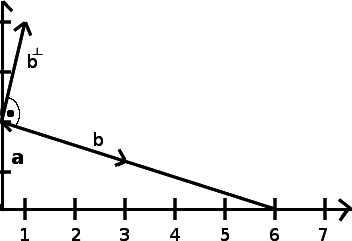
\includegraphics[width=0.3\textwidth]
	{mainmatter/chapter1/pics/orthovek.png}
	\caption{Gerade mit orthogonalen Vektor} 
\end{figure}



\subsection{Satz 1.2}
Eine Teilmenge von $\mathbb{R}^{2}$ ist eine Gerade genau dann, wenn sie Lösungsmenge einer Gleichung \\
$\{\begin{pmatrix}x \\ y \end{pmatrix} \in \mathbb{R}^{2} : \alpha x + \beta y = \gamma\}$ ist. $\alpha$ und $\beta$ nicht beide Null.
%
%
%
\subsubsection{Beweis:}
$l=a + \mathbb{R}b$\\
Dann erfüllt jeder Punkt $(a_{1}+tb_{1},a_{2}+tb_{2})$ die Gleichung $b_{2}a_{1}-b_{1}a_{2} = b_{2}x-b_{1}y$.\\
DENN:  $b_{2}(a_{1}+tb_{1})-b_{1}(a_{2}+tb_{2})=b_{2}a_{1}-b_{1}a_{2}=det(a,b)$ Erfüllt umgekehrt $\begin{pmatrix}x \\ y \end{pmatrix}$ die Gleichung $\alpha x + \beta y = \gamma$ und ist $\alpha \neq 0$, dann folgt $x=\frac{-\beta}{\alpha}y+\frac{\gamma}{\alpha}$. \\ 
Also ist $\begin{pmatrix}x \\ y \end{pmatrix}$ ein Punkt der Geraden $a + \mathbb{R}b$ mit $a=\begin{pmatrix} \frac{\gamma}{\alpha} \\ 0 \end{pmatrix}, b=\begin{pmatrix} -\beta \\ \alpha \end{pmatrix}$\\
%
%
%
\subsubsection{Beispiel:} 
\begin{equation*}
x-y=1 \qquad a=\begin{pmatrix} 1 \\ 0 \end{pmatrix} b=\begin{pmatrix} 1 \\ 1 \end{pmatrix}
\end{equation*}
\begin{figure}[H]
	\centering
	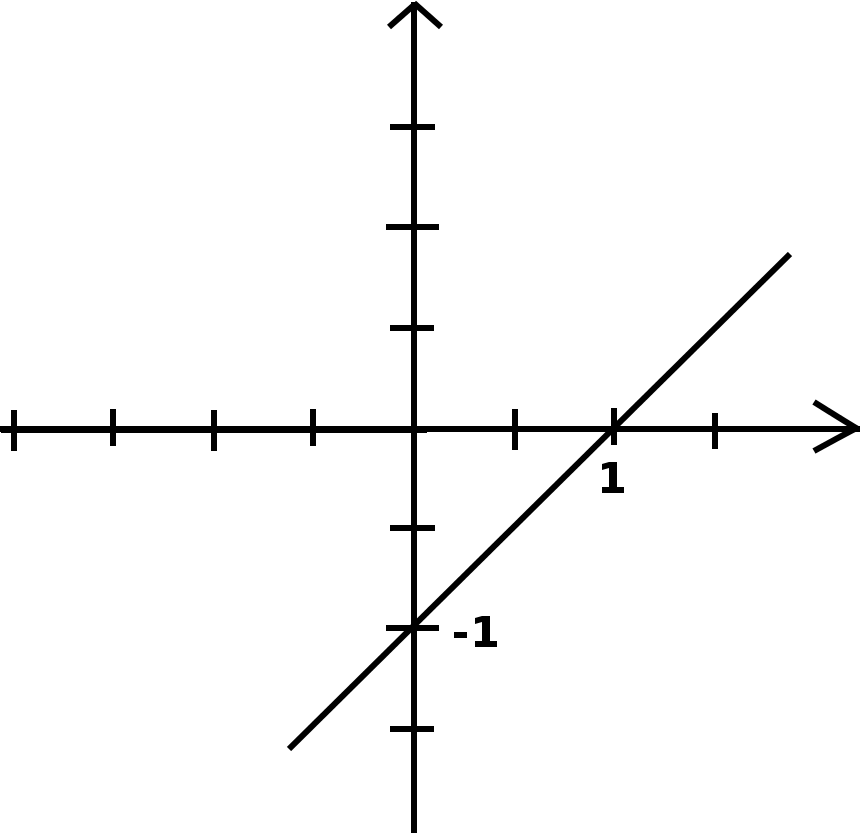
\includegraphics[width=0.3\textwidth]
	{mainmatter/chapter1/pics/bsp12.png}
	\caption{Beispiel zu Satz 1.2} 
\end{figure}
	\section{Lineare Abbildungen}
$A: \mathbb{R}^{2} \rightarrow \mathbb{R}^{2}$ heißt linear, wenn für jedes $a,b \in \mathbb{R}^{2}$ gilt: $A(x\vec{a} + y \vec{b})=xA(\vec{a}) + yA(\vec{b})$\\

$A\begin{pmatrix} 1\\0 \end{pmatrix}$ und $A\begin{pmatrix} 0 \\ 1 \end{pmatrix}$ können beliebig vorgegeben werden. Anderseits ist $A$ durch diese bestimmt.\\

$A\begin{pmatrix} x \\ y \end{pmatrix}= x\cdot A\begin{pmatrix} 1 \\ 0 \end{pmatrix} + y \cdot A\begin{pmatrix} 0 \\ 1 \end{pmatrix}$ \\

$A\begin{pmatrix}1 \\ 0 \end{pmatrix} = \begin{pmatrix} a_{1} \\ a_{2} \end{pmatrix} \qquad A\begin{pmatrix} 0 \\ 1 \end{pmatrix} = \begin{pmatrix} b_{1} \\ b_{2} \end{pmatrix}$ \\

$A\begin{pmatrix} x \\ y \end{pmatrix} = \mathop{\underbrace{\begin{pmatrix} a_{1} & b_{1} \\ a_{2} & b_{2} \end{pmatrix}}}\limits_{(2\times 2) - \textrm{Matrix}} \cdot \begin{pmatrix} x \\ y \end{pmatrix} \coloneq \begin{pmatrix} a_{1}x + b_{1} y \\ a_{2}x + b_{2}y\end{pmatrix} = xa+by$\\
Eigenschaft: Die erste Spalte von $A$ ist ist der Bildvektor von $\begin{pmatrix}1 \\ 0 \end{pmatrix}$
%
%
%
\subsubsection{Beispiel: }
$\begin{pmatrix} 1 & 0 \\ 0 & 1 \end{pmatrix}$ repräsentiert die identische Abbildung.
%
%
%
\subsubsection{Satz: }
sind $A,B: \mathbb{R}^{2}\rightarrow \mathbb{R}^{2}$ linear, so auch die Verknüpfung $A \circ B$.
%
%
%
\subsubsection{Beweis:}
$A(B(xa+yb))=A(xB(a)+yB(b))=xAB(a)+yAB(b)$\\
Komposition linearer Abbildungen:\\
$A=\begin{pmatrix} a_{1} & b_{1} \\ a_{2} & b_{2} \end{pmatrix}; \ B=\begin{pmatrix} c_{1} & d_{1} \\ c_{2} & d_{2} \end{pmatrix}$ \\
$A \circ B \ \begin{pmatrix}x_{1} \\ x_{2} \end{pmatrix} = \begin{pmatrix}a_{1} & b_{1} \\ a_{2} & b_{2} \end{pmatrix} \cdot \begin{pmatrix} c_{1}x_{1} + d_{1} x_{2} \\ c_{2}x_{1} + d_{2}x_{2} \end{pmatrix} = \begin{pmatrix} a_{1}c_{1}x_{1} + a_{1}d_{1}x_{2} & b_{1}c_{1}x_{1} + b_{1}d_{1}x_{2} \\ a_{2}c_{1}x_{1} + a_{2}d_{1}x_{2} & b_{2}c_{2}x_{1} + b_{2} d_{2}x_{2} \end{pmatrix} = \begin{pmatrix} a_{1} c_{1} + c_{2} b_{1} & a_{1} d_{1} + b_{1} d_{2} \\ a_{2} c_{1} + b_{2} c_{2} & a_{2}d_{1} + b_{2}d_{2} \end{pmatrix} \ \begin{pmatrix} x_{1} \\ x_{2} \end{pmatrix}$\\
\qquad\\
\qquad\\
$\begin{pmatrix} \textcolor{pred}{a_{1}} & \textcolor{pred}{b_{1}} \\ \textcolor{pviolet}{a_{2}} & \textcolor{pviolet}{b_{2}}\end{pmatrix} \cdot \begin{pmatrix} \textcolor{pgreen}{c_{1}} & \textcolor{pblue}{d_{1}} \\ \textcolor{pgreen}{c_{2}} & \textcolor{pblue}{d_{2}}\end{pmatrix} = \begin{pmatrix}\textcolor{pred}{a_{1}}\textcolor{pgreen}{c_{1}} + \textcolor{pred}{b_{1}}\textcolor{pgreen}{c_{2}}  & \textcolor{pred}{a_{1}}\textcolor{pblue}{d_{1}} + \textcolor{pred}{b_{1}}\textcolor{pblue}{d_{2}} \\ \textcolor{pviolet}{a_{2}}\textcolor{pgreen}{c_{1}}+\textcolor{pviolet}{b_{2}}\textcolor{pgreen}{c_{2}} & \textcolor{pviolet}{a_{2}} \textcolor{pblue}{d_{1}} + \textcolor{pviolet}{b_{2}}\textcolor{pblue}{d_{2}}\end{pmatrix}$\\
\qquad\\
\begin{figure}[H]
	\centering
	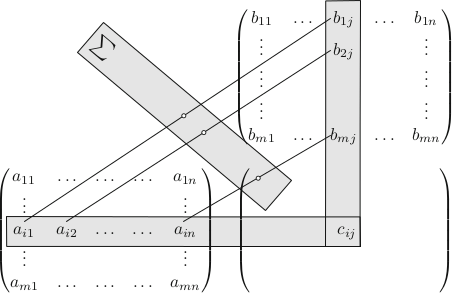
\includegraphics[width=0.5\textwidth]
	{mainmatter/chapter1/pics/matrixmult.png}
	\caption{Schema der Matrixmultiplikation} 
\end{figure}
Matrixmultiplikation entspricht Komposition von Abbildungen\\
Sie ist im Allgemeinen nicht Kommutativ.\\
\qquad\\
$\begin{pmatrix} 1 & 2 \\ 3 & 4 \end{pmatrix} \cdot \begin{pmatrix} 5 & 6 \\ 7 & 8 \end{pmatrix} = \begin{pmatrix} 1 \cdot 5 + 2 \cdot 7 & 1 \cdot 6 + 2 \cdot 8 \\ 3 \cdot 5 + 4 \cdot 7 & 3 \cdot 6 + 4 \cdot 8\end{pmatrix} = \begin{pmatrix} 19 & 22 \\ 43 & 50 \end{pmatrix}$ \\
.\qquad \qquad \qquad \qquad \qquad \qquad \qquad$ \neq $\\
$\begin{pmatrix} 5 & 6 \\ 7 & 8 \end{pmatrix} \cdot \begin{pmatrix} 1 & 2 \\ 3 & 4 \end{pmatrix}= \begin{pmatrix} 5 \cdot 1 + 6 \cdot 3 & 5 \cdot 2 + 6 \cdot 4 \\ 7 \cdot 1 + 8 \cdot 2 & 7 \cdot 2 + 8 \cdot 4 \end{pmatrix} = \begin{pmatrix} 23 & 34 \\ 23 & 46 \end{pmatrix}$\\
%
%
%
\subsubsection{Satz:}
Matrixmultiplikation ist assoziativ.
%
%
%
\subsubsection{Beweis:} 
$(A\cdot B) \cdot C = A \cdot (B \cdot C)$ \\
Interpretiere $A,B,C$ als Abbildungen\\
$A\circ (B \circ C) (a) = A\circ B (C(a)) = A(B(C(a)))$\\
$(A\circ B) \circ C (a)=(A\circ B)C(a)=A(B(C(a)))$
%
%
%
\subsubsection{Satz:}
$A: \mathbb{R}^{2} \rightarrow \mathbb{R}$ lineare Abbildungen\\
$A$ ist injektiv $\Leftrightarrow A$ ist surjektiv
%
%
%
\subsubsection{Beweis:}
$Ax=b$ \\
Existenz von $x \Leftrightarrow$ Surjektivität\\
Eindeutigkeit von $x \Leftrightarrow$ Injektivität\\
$det A \neq 0 \Leftrightarrow A$ injektiv $\Leftrightarrow A$ surjektiv. \\
/* Durch Benutzung der Cramerschen Regel */
	\section{Inverse Matrix, Basiswechsel}
Ist $A=\begin{pmatrix}a_{1} & b_{1} \\ a_{2} b_{2} \end{pmatrix}$ und $\lambda \in \mathbb{R}: \ \lambda \cdot A = \begin{pmatrix} \lambda a_{1} & \lambda b_{1} \\ \lambda a_{2} & \lambda b_{2} \end{pmatrix}$\\
%
%
%
\subsubsection{Satz:}
Für $A=\begin{pmatrix}a_{1} & b_{1} \\ a_{2} b_{2} \end{pmatrix}$ mit $det(A) \neq 0$ gilt:\\
$A^{-1} = \frac{1}{det(a)} \cdot \begin{pmatrix} b_{2} & -b_{1} \\ -a_{2} & a_{1} \end{pmatrix}$
%
%
%
\subsubsection{Beweis:}
$A\cdot A^{-1} = \begin{pmatrix}a_{1} & b_{1} \\ a_{2} b_{2} \end{pmatrix} \cdot \frac{1}{det(a)} \cdot \begin{pmatrix} b_{2} & -b_{1} \\ -a_{2} & a_{1} \end{pmatrix}$\\
$ = \frac{1}{det(a)} \cdot \begin{pmatrix} det(A) & 0 \\ 0 & det(A) \end{pmatrix}$\\
$= \begin{pmatrix} 1 & 0 \\ 0 & 1 \end{pmatrix}$\\
$A^{-1}\cdot A$ analog $\Rightarrow A^{-1} \cdot A = \begin{pmatrix} 1 & 0 \\ 0 & 1 \end{pmatrix}$ \\
$\mathcal{B} = (\vec{b_{1}}, \vec{b_{2}})$ Basis $ \leadsto \begin{pmatrix} b_{11} & b_{21} \\ b_{12} & b_{22} \end{pmatrix} = B$\\
$\vec{a} = x_{1}\vec{b_{1}} = B\vec{x} : \vec{x} = B^{-1}\vec{a}$\\
Die Koordinaten von $a$ bzgl. $B$ sind durch $B^{-1}(\vec{a})$ gegeben.
	\section{Satz von Pythagoras, Länge und Skalarprodukt}
		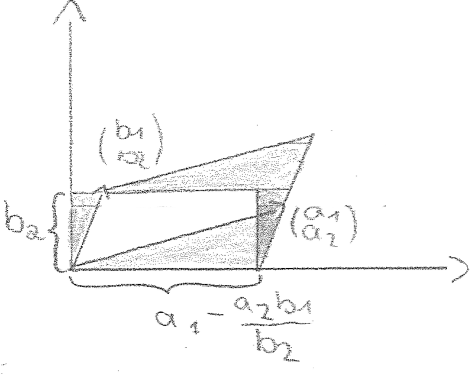
\includegraphics[width=0.35\textwidth]
	{mainmatter/chapter1/pics/parallelogram.png}Fläche des Parallelogramms gleich $|det(\vec{a},\vec{b})|$\\
$\begin{pmatrix} a_{1} \\ a_{2} \end{pmatrix} + \lambda \begin{pmatrix} b_{1} \\ b_{2} \end{pmatrix} = \begin{pmatrix} x \\ 0 \end{pmatrix} \mathop{\Rightarrow}\limits^{b_{2} \neq 0} \lambda = \frac{-a_{2}}{b_{2}}, x=a_{1}-\frac{a_{2}b_{1}}{b_{2}}$ \\
Rechteck hat Fläche $\vert a_{1}b_{2}-a_{2}b_{1}\vert=\vert det(a,b) \vert =$ Fläche des Parallelogramms. 
%
%
%
\subsection{Satz des Pythagoras (1. Version)}
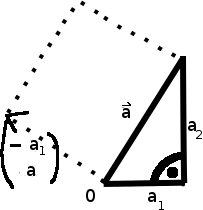
\includegraphics[width=0.15\textwidth]
	{mainmatter/chapter1/pics/pyth.png}$\vec{a} = \begin{pmatrix} a_{1} \\ a_{2} \end{pmatrix}$ hat Länge $\Vert \vec{a} \Vert = \sqrt{a_{1}^{2} + a_{2}^{2}}$
%
%
%
\subsubsection{Beweis:}
$det(\vec{a},\vec{a}_{\perp})=a_{1}^{2+}a_{2}^{2}$ ist das Quadrat der Seitenlänge $\sqrt{a_{1}^{2}+a_{2}^{2}}$
%
%
%
\subsubsection{Definition:}
Der Abstand zweier Vektoren $\vec{a}$ und $\vec{b}$ ist $ \qquad \Vert \vec{a}-\vec{b} \Vert$
%
%
%
\subsubsection{Bemerkung:}
$\begin{pmatrix} a_{1} \\ a_{2} \end{pmatrix} \perp \begin{pmatrix} b_{1} \\ b_{2} \end{pmatrix} \Rightarrow \begin{pmatrix} b_{1} \\ b_{2} \end{pmatrix} = \lambda \begin{pmatrix} -a_{2} \\ a_{1} \end{pmatrix} \Leftrightarrow a_{1}b_{1}+a_{2}b_{2}=0$
\begin{description}
	\item["`$\Rightarrow$"'] $a_{1}b_{1}+a_{2}b_{2}= -\lambda a_{1}a_{2} + \lambda 
		a_{1}a_{2}$
	\item["`$\Leftarrow$"'] Falls $ a = \begin{pmatrix} 0 \\ 0 \end{pmatrix} \leadsto 
		\lambda = 0$ \\ 
		o.E. $a_{1} \neq 0 $ \\
		setze $\lambda: b_{2} = \lambda a_{1} \mathop{\Rightarrow}\limits^{\text{Vor.}} 
		0 = a_{1}b_{1}+ a_{1}\cdot\lambda a_{1}a_{2} \Rightarrow b_{1} = - 
		\lambda a_{2}$
\end{description}
%
%
%
\subsubsection{Definition:}
Skalarprodukt\\
Das von $\vec{a}$ und $\vec{b}: <\vec{a},\vec{b}> = a_{1}b_{1}+a_{2}b_{2}$.
%
%
%
\subsubsection{Eigenschaften des Skalarprodukts}
$<\vec{a}+\vec{b},\vec{c}>=(a_{1}+b_{1})c_{1}+(a_{2}+b_{2})c_{2}=<a,c>+<b,c>$\\
$<\lambda \vec{a},\vec{b}>=\lambda <\vec{a},\vec{b}>$\\
$<\vec{a},\vec{b}>=<\vec{b},\vec{a}>$
%
%
%
\subsection{Pythagoras (allgemein)}
$\vec{a}\perp\vec{b} \Rightarrow \Vert \vec{a} - \vec{b} \Vert^{2} = \Vert \vec{a} \Vert^{2} + \Vert \vec{b} \Vert ^{2}$
%
%
%
\subsubsection{Beweis:}
$<\vec{a},\vec{b}>=0 $\\
$\Vert \vec{a} - \vec{b} \Vert^{2} = (a_{1}-b_{1})^{2} + (a_{2} - b_{2})^{2} = a_{1}^{2}+b_{1}^{2}+a_{2}^{2}+b_{2}^{2} = \Vert \vec{a} \Vert^{2} + \Vert \vec{b} \Vert^{2}$
%
%
%
\subsection{Satz des Thales}
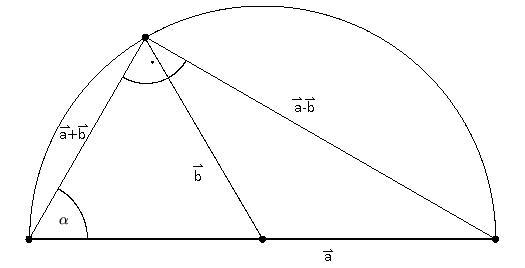
\includegraphics[width=0.5\textwidth]
	{mainmatter/chapter1/pics/satzdesthales.png}\\
	
$\vec{a},\vec{b}: \Vert \vec{a} \Vert =\Vert \vec{b} \Vert \Rightarrow \vec{a} - \vec{b} \perp  \vec{a} + \vec{b}$
%
%
%
\subsubsection{Beweis:}
$<\vec{a}-\vec{b},\vec{a} + \vec{b}> = <\vec{a},\vec{b}>-<\vec{b},\vec{a}>+<\vec{a},\vec{a}>-<\vec{b},\vec{b}>=0$
%
%
%
\subsubsection{Satz:}
Sei $l$ Gerade, $c \notin l$. \\
Dann existiert genau ein "`Fußpunkt"' $D \in l: c-D\perp l$
%
%
%
\subsubsection{Beweis:}
$\vec{n} \perp l$. Schneide $c+ \mathbb{R}\vec{n}$  mit $l$. \\
$det(\vec{n},\vec{n}^{\perp})=\Vert \vec{n}\Vert^{2} \neq 0 \Rightarrow$ es existiert $D$ 
%
%
%
\subsubsection{Höhensatz}
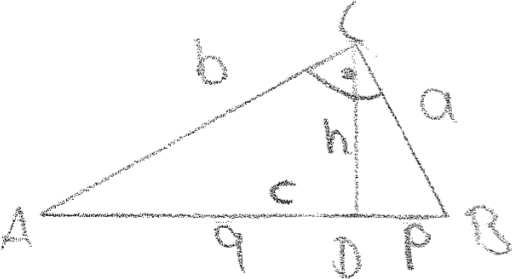
\includegraphics[width=0.3\textwidth]
	{mainmatter/chapter1/pics/heohensatz.png}\\
	$ABC$ sei ein rechtwinkliges Dreieck
	$p=\Vert D-B \Vert \qquad q=\Vert D-A\Vert \qquad h=\Vert D-C\Vert \Rightarrow h^{2}=pq$
%
%
%
\subsubsection{Beweis:}
$a^{2} + b^{2} = c^{2} = p^{2} + 2pq + q^{2}$\\
$a^{2}=h^{2}+p^{2}$\\
$b^{2}=h^{2}+q^{2}$\\
\qquad\\
$\Rightarrow p^{2} + 2pq +q^{2} = 2h^{2}+p^{2}+q^{2}$\\
$\Leftrightarrow 2pq = 2h^{2}$\\
$\Leftrightarrow pq=h^{2} \qquad \square$
%
%
%
\subsubsection{Kathetensatz}
$ABC$ sei ein rechtwinkliges Dreieck
$a^{2} = p\cdot c, b^{2} = q\cdot c$
%
%
%
\subsubsection{Beweis:}
$a^{2} = c^{2}-b^{2}=p^{2}+2pq+q^{2}-(h^{2}+q^{2})=p^{2}+2pq-h^{2}=p^{2}+2pq-a^{2}+p^{2}$\\
\qquad\\
$2a^{2}=2pq+2p^{2}$\\
$\Leftrightarrow a^{2} = pq+p^{2} \Rightarrow$ Behauptung; analog für $b^{2} = qc \qquad\square$
	\section{Bewegungen}
%
%
%
\subsubsection{Definition:}
Eine Abbildung heißt Bewegung oder Isometrie wenn $\forall a,b \in \mathbb{R}^{2}\qquad \Vert A(c) - A(b) \Vert = \Vert \vec{a}-\vec{b}\Vert$.
%
%
%
\subsubsection{Satz:}
$A: \mathbb{R}^{2} \rightarrow \mathbb{R}^{2}$ Bewegung mit $A\begin{pmatrix} 0 \\ 0 \end{pmatrix} = \begin{pmatrix} 0 \\ 0 \end{pmatrix}$. Dann ist $A$ linear. Es gibt $c,s \in \mathbb{R}$ mit $c^{2}+s^{2}=1$, sodass die Matrix von $A \, R_{c,s} = \begin{pmatrix} c & -s \\ s & c \end{pmatrix} \, det(R_{c,s}) = 1$ oder $S_{c,s} = \begin{pmatrix} c & s \\ s & -c \end{pmatrix} \, det(S_{c,s}) = -1$
%
%
% Grafiken einfügen
%
%
\subsubsection{Beweis:}
$A$ ist Isometrie.\\
$A\begin{pmatrix} 1 \\ 0 \end{pmatrix} = \begin{pmatrix} c \\ s \end{pmatrix}  \quad A\begin{pmatrix} 0 \\ 1 \end{pmatrix} = \begin{pmatrix} t \\ u \end{pmatrix} \quad A\begin{pmatrix} x \\ y \end{pmatrix} = \begin{pmatrix} z \ w \end{pmatrix}$\\
$ c^{2}+s^{2}=1=t^{2}+u^{2}$\\
$(c-t)^{2} + (s-u)^{2} = 2 = c^{2}  = 2 + c + t^{2} + s^{2} - 2su+u^{2}$ \Huge{\textcolor{red}{?}}\normalsize{} \\
$=2-2\mathop{\underbrace{(tc+su)}}\limits_{\Rightarrow 0 }$\\
$\Rightarrow \begin{pmatrix} t \\ u \end{pmatrix} = \lambda \begin{pmatrix} -s \\ c \end{pmatrix}, \lambda = \pm 1$\\
$A$ linear: z.z. $\begin{pmatrix}z \\ w \end{pmatrix} = \begin{pmatrix} xx \pm sy \\ sx \pm cy \end{pmatrix} x^{2}+y^{2} = z^{2} + w^{2}$\\
$(x-1)^{2} + y^{2} \mathop{=}\limits^{\text{\RM{1}}} ( z-c)^{2} + (w-s)^{2}$\\
$\Leftrightarrow x^{2}-2x+1+y^{2} = z^{2}-2zc+c^{2}+w^{2}-2sw+s^{2}$\\
$\Rightarrow x= cz + sw$\\
$(z+s)^{2} + (w-c)^{2} = x^{2}+(y-1)^{2}$\\
$\Leftrightarrow 2sz-2cw = -2y$\\
$\Rightarrow y = -sz$\\
	\section{Isometrie}
$A: \mathbb{R}^{2} \rightarrow \mathbb{R}^{2}$\\
$\Vert Av \Vert = \Vert v \Vert$\\
\qquad\\
 \begin{tabular}{c|c}
 	Drehung & Spiegelung \\ \hline
  	$det(a) = 1$ & $det(A) = 1$ \\ 
  	$R_{c,s}=\begin{pmatrix} c & -s \\ s & c \end{pmatrix}$ & $S_{c,s} = \begin{pmatrix} c & s \\ s & -c \end{pmatrix}$\\
 	$c^{2}+s^{2} = 1$ & $c^{2}+s^{2} = 1$\\
 \end{tabular}
 %
 %
 %Grafik einfügen
 %
 %
 \subsubsection{Definition (Winkel):}
 Sind $a,b \in \mathbb{R}^{2}\diagdown \{0\}$ Vektoren dann heißt die eindeutige Drehung $\alpha =R_{c,s}$ mit $\alpha(a)=\lambda\cdot b, \, \lambda \in \mathbb{R}_{\geq 0}$ der Winkel zwischen $a$ und $b$, und wir schreiben $\alpha := < (a,b)$\\
 Die Summe $\alpha + \beta$ zweier Winkel $\alpha$ und $\beta$ definieren wir als $\alpha + \beta := \alpha \circ \beta$ (beachte $\alpha + \beta = \beta + \alpha$)\\
 Das negative eines Winkels $\alpha$ definieren wir als $-\alpha := \alpha ^{-1}$ d.h. ist $\alpha = R_{cs} \Rightarrow \alpha^{-1} = R_{c,-s}$ Sind $A,B,C \in \mathbb{R}^{2}$ Punkte, dann definieren wir den Winkel an Punkt $A$ des Tripels $(ABC)$ als < $(B,A,C) := < (B-A,C-A)$. 
 %
 %
 %
 \subsubsection{Definition (Winkelhalbierende):}
 Ist $\alpha$ ein Winkel, dann existiert ein Winkel $\beta$ mit $\beta + \beta = \alpha$. Dieser heißt der halbe Winkel zu $\alpha$ oder auch die Winkelhalbierende zu $\alpha$.
 %
 %
 %
 \subsubsection{Satz:}
 Ist $\alpha = R_{c,s}$ so kann man $\beta = R_{t,u}$ wählen mit \\
 $t = \pm \sqrt{\frac{1}{2}(1+c)}, \, u=\sqrt{\frac{1}{2}(1-c)}$ wobei $"`+"' \Leftrightarrow s \geq 0$. 
 %
 %
 %
 \subsubsection{Beweis:}
 Nehmen wir an, dass $\alpha = 2 \beta$ mit $\alpha = \begin{pmatrix} c & -s \\ s & c \end{pmatrix}, \, \beta = \begin{pmatrix} t & -u \\ u & t \end{pmatrix}$\\
 $\Rightarrow \begin{pmatrix} c & -s \\ s & c \end{pmatrix} = \begin{pmatrix} t & -u \\ u & t \end{pmatrix} \begin{pmatrix} t & -s \\ u & t \end{pmatrix} = \begin{pmatrix} t^{2}-u^{2} & -2tu \\ 2tu & t^{2}-u^{2} \end{pmatrix}$\\
 \qquad\\
 Es gilt also $c=t^{2}-u^{2}, \, s=2tu$\\ 
 \qquad\\
$
\begin{array}{rcrcr}
c \cdot 4t^{2} &=& 4t^{4} &-& 4u^{2}t^{2}\\
 &=& 4t^{4} &-&  s^{2}\\
 &=& 4t^{4} &-& (1-c^{2})
\end{array} 
$\\
\qquad\\
\qquad\\
$ \Rightarrow t^{4} - c\cdot t^{2} - \frac{1}{4}(1-c^{2})=0$\\
$\mathop{\Rightarrow}\limits^{\text{pq}}t^{2} = \frac{c}{2} \pm \sqrt{\frac{c^{2}}{4}+\frac{1}{4}(1-c^{2})} = \frac{c}{2} \pm \frac{1}{2}=\frac{1}{2}(c\pm 1) \geq 0$\\
\qquad\\
Wir wissen $1=c^{2}+s^{2}\geq 0 \Rightarrow  -1 \leq c \leq 1$\\
wegen $1=t^{2}+u^{2}\Rightarrow 0 \leq t^{2}\leq 1$\\
Würden oben ein "`-"' stehen, wäre $t^{2} < 0$ für $c<0 \lightning$\\
$\Rightarrow t^{2} = \frac{1}{2}(c+1) \Rightarrow t = \pm \sqrt{\frac{1}{2}(c+1)}$\\
Analog folgt $u=\sqrt{\frac{1}{2}(1-c)}$ \\
$t^{2}-u^{2} = \frac{1}{2}(c+1)-\frac{1}{2}(1-c)=\frac{1}{2}c + \frac{1}{2}c = c$\\
$2tu=2\cdot(\pm\sqrt{\frac{1}{2}(1+c)\cdot\frac{1}{2}(1-c)} = \pm 2 \sqrt{\frac{1}{4}\mathop{\underbrace{(1-c^{2})}}\limits_{s^{2}}} = \pm \sqrt{s^{2}} = \pm \vert s \vert \mathop{=}\limits^{\text{!}} s$\\
Die letzte Gleichheit gilt genau dann, wenn $\pm$ das Vorzeichen von $s$ ist (d.h. "`+"' $\Leftrightarrow \, s \geq 0$).\\
\qquad\\
Wir messen Winkel, indem wir der Drehung $\begin{pmatrix} -1 & 0 \\ 0 & -1 \end{pmatrix}$ den Wert 180$^{\circ}$ oder $\pi$ zu.\\
Durch das Halbieren und Addieren von Winkeln können wir jeden Winkel eine Zahl $0^{\circ} \leq x \leq 360^{\circ}$ zuordnen, die wir das Winkelmaß nennen. \\
z.B. $\frac{1}{3} = \sum\limits^{\infty}_{n=1} \frac{1}{4^{n}}$\\
Tatsächlich lässt dich jede Zahl $ 0 \leq x \leq 360 $ schreiben als $360^{\circ} \cdot  \sum\limits^{\infty}_{n=1}a_{n}\frac{1}{2^{n}}, \qquad a_{n}\in  \mathbb{N}_{0}$ \\
Was ist der halbe Winkel zu $\begin{pmatrix} -1 & 0 \\ 0 & -1 \end{pmatrix}$ ?\\
$R_{t,u}$ mit $t = \pm \sqrt{\frac{1}{2}(1+c)} = 0 \, u = \sqrt{\frac{1}{2}(1-c)} = 1$ d.h. $R_{t,u} = \begin{pmatrix} 0 & 1 \\ 1 & 0 \end{pmatrix} \mathrel{\widehat{=}} 90^{\circ} = \mathop{\alpha}\limits^{\text{\RM{2}}}$
%
%
%
\subsubsection{Satz (Winkelsumme im Dreiecke):}
Es sei $a,b,c$ ein Dreieck (d.h. $a,b,c$ sind Punkte) und $\alpha := \measuredangle ( b,a,c), \, \beta := \measuredangle(c,b,a), \, \gamma := \measuredangle (a,c,b)$\\
Dann gilt $\alpha + \beta + \gamma = 180^{\circ} (=\pi)$
%
%
%
\subsubsection{Beweis:}
$\alpha(b-a)=\lambda(c-a), \, \lambda \in \mathbb{R}_{>0}$\\
$\beta(c-b)=\mu(c-b), \, \mu \in \mathbb{R}_{>0}$\\
$\gamma(a-c)= r(a-c), \, r \in \mathbb{R}_{>0}$\\
\qquad\\
$
\begin{array}{rcr}
(\alpha + \beta + \gamma)(a-c) &\mathop{=}\limits^{\text{Definition}}& \alpha \circ \beta \circ \gamma(a-c)\\
 &=&  \alpha (\beta(\gamma(a-c)))\\
 &=& \alpha(\beta(r(b-c)))\\
 &=& \alpha (\beta(-r(c-b)))\\
 &=& -r \cdot \alpha(\beta(c-b))\\
 &=& -r\cdot \alpha(\mu(a-b))\\
 &=& \mu \cdot r \cdot \alpha (b-a)\\
 &=& -\alpha \mu r (a-c)
\end{array} 
$\\
Da $\alpha + \beta + \gamma$ wieder eine Drehung ist, gilt $\Vert a-c\Vert = \Vert (\alpha + \beta + \gamma)(a-c)\Vert=\vert\lambda \mu r\vert \cdot \Vert (a-c)\Vert \Rightarrow \vert \lambda \mu r\vert=1$\\
Da $\alpha, \mu, r > 0 \Rightarrow \lambda\mu r = 1$\\
Somit gilt \\
($\alpha+\beta+\gamma)(a-c)=-\lambda \mu r (a-c) = -1(a-c)=\begin{pmatrix} -1 & 0 \\ 0 & -1\end{pmatrix}(a-c) \Rightarrow \alpha + \beta + \gamma=180^{\circ} \rightarrow$ Drehung $\square$
%
%
%
\subsubsection{Korollar:}
In einem Viereck ist die Summe der Innenwinkel $360^{\circ}$
%
%
%
\subsubsection{Beweis:}
Zerlege das Viereck durch verbinden zweier nicht verbundenen Ecken in 2 Dreiecke:
%
%
% Grafik einfügen
%
%
\subsubsection{Satz(Gleichschenklige Dreiecke):}
Sei $a,b,c$ ein gleichschenkliges Dreieck, d.h. $\Vert a-c \Vert = \Vert b-c \Vert$, dann gilt $\measuredangle (b,a,c) = \measuredangle (c,b,a)$
%
%
%Grafik einfügen
%
%
\subsubsection{Beweis:}
o.E. gilt $c=0$\\
Dann gilt also $a-c=a, \, b-c=b$.\\
Es sei $d:=a+b$. \\
\qquad\\
Behauptung:\\
 $a+b\perp a-b$\\
 \qquad\\
Beweis:\\
$<a+b,a-c>=<a,a>+<b,a>-<a,b>-<b,b>=\Vert a \Vert^{2}-\Vert b \Vert^{2} = 0$ nach Voraussetzung $\Vert a \Vert = \Vert b \Vert$\\
%
%
%Grafig einfügen
%
%
$m:=\frac{1}{2}(a+b)$\\
$\alpha + \gamma_{1} - \frac{\pi}{2}=\pi \Rightarrow \alpha + \gamma_{1} = \frac{\pi}{2}$\\
$\beta+\gamma_{2}+\frac{\pi}{2}=\pi\Rightarrow\beta+\gamma_{2}\frac{\pi}{2}$\\
Wir zeigen $\gamma_{1}=\gamma_{2}$ indem wir zeigen, dass $m$ auf der Winkelhalbierenden von $\gamma$ liegt. \\
$R(\vec{a})=\lambda b$\\
$R_{\gamma}=\begin{pmatrix} c & -s \\ s & c \end{pmatrix}$\\
$R_{\frac{\gamma}{2}}=\begin{pmatrix} \sqrt{\frac{1}{2} (1+c)} & - \sqrt{\frac{1}{2}(1-c)} \\ \sqrt{\frac{1}{2}(1-c)} & \sqrt{\frac{1}{2}(1+c)}\end{pmatrix} \qquad u=\sqrt{\frac{1}{2}(1-c)}$\\
$\lambda :=\sqrt{\frac{1}{2}(1+c)}$\\
$\lambda \cdot R_{\frac{\gamma}{2}} \cdot \vec{u} = \begin{pmatrix} \frac{1}{2} (1+c)a_{1} -\frac{1}{2}\sqrt{1-c^{2}}a_{2} \\ \frac{1}{2}\sqrt{1-c^{2}}a_{1} + \frac{1}{2}(1+c)a_{2}\end{pmatrix}$\\
$= \frac{1}{2}(\begin{pmatrix}a_{1} \\ a_{2} \end{pmatrix} + R_{\gamma} \begin{pmatrix} a_{1} \\ a_{2} \end{pmatrix} ) = \frac{1}{2}(\vec{a}+\vec{b}=\vec{m}$\\
$\vec{m}$ liegt also auf der Winkelhalbierenden von $\Rightarrow \gamma_{1} = \gamma_{2} = \frac{\gamma}{2}$


%		 \chapter{Der Raum $\mathbb{R}^{3}$}
	%
%
%
Elemente $\vec{a} = \begin{pmatrix}a_{1} \\ a_{2} \\ a_{3} \end{pmatrix}$
 wie in $\mathbb{R}^{2}$: Addition, skalare Multiplikation. \\
%
%
%
\subsubsection{Definition:}
$a \in \mathbb{R}^{3}$:
\begin{enumerate}
 \item Länge von a \quad $\left\Vert\vec{a}\right\Vert = \sqrt{a_{1}^{2} + a_{2}^{2} + a_{3}^{2}}$ 
 \item ${<}\vec{a}, \vec{b}{>} = a_{1}b_{1} + a_{2}b_{2} + a_{3}b_{3}$
 \item $ \vec{a}$ und $\vec{b}$ linear abhängig $\vec{b} = t\vec{a}$ oder $\vec{a} = t\vec{b}$.\\
 linear unabhängig $\mathop{\Leftrightarrow}\limits^{\text{Definition}}$ nicht linear abhängig.
\end{enumerate}
%
%
%
\subsubsection{Rechenregeln:}
\begin{enumerate}
 \item ${<}\vec{a}, \vec{b}{>} = {<}\vec{b}, \vec{a}{>}$
 \item ${<}\vec{a} + \vec{b}, \vec{c}{>} = <\vec{a}, \vec{c}> + <\vec{b}, \vec{c}>$ (Bilinearität)
 \item $<\lambda\vec{a}, \vec{b}> = \lambda <\vec{a}, \vec{b}>$
 \item $<\vec{a}, \vec{a}> = \left\Vert\vec{a}\right\Vert^{2}$
\end{enumerate}
%
%
%
\subsubsection{Satz:}
$\vec{a},\vec{b} \in \mathbb{R}^3$ $(\vec{a} \neq \vec{0}, \vec{b} \neq \vec{0})$, 
Dann ist $\vec{p}=\frac{<\vec{a},\vec{b}>}{\left\Vert\vec{a}\right\Vert^{2}} \cdot\vec{a}$
ist der eindeutig bestimmte Punkt auf $\mathbb{R}\vec{a}$ mit minimalem Abstand zu $\vec{b}$ Es gilt:
$ \left\Vert\vec{b}\right\Vert^{2} - \left\Vert\vec{p}\right\Vert^{2} + \left\Vert\vec{b} - \vec{p}\right\Vert^{2}$
%
% Bild einfügen
%
\subsubsection{Beweis}
$\left\Vert t\vec{a} - \vec{b}\right\Vert^{2} = \, <t\vec{a} - \vec{b}, t\vec{a} - \vec{b}>$
\begin{description}
 \item [\tab] $ = t^{2}<\vec{a}, \vec{a}> - 2t<\vec{a}, \vec{b}> + <\vec{b}, \vec{b}>$
 \item [\tab] $ = \left( \Vert a \Vert t - \frac{<\vec{a}, \vec{b}>}{\Vert a \Vert}\right)^{2} + <\vec{b}, \vec{b}> - \frac{<{\vec{a}, \vec{b}>}^2}{\left\Vert\vec{a}\right\Vert^{2}}$
\end{description}
Minimum: $ t = \frac{<\vec{a}, \vec{b}>}{\left\Vert\vec{a}\right\Vert^2}$
ergibt den Wert $\left\Vert\vec{b}\right\Vert^2 - \frac{<\vec{a}, \vec{b}>^2}{\left\Vert\vec{a}\right\Vert^2}$\\
$\cos\varphi = \frac{Ankathete}{Hypothenuse} = \frac{\left\Vert\vec{p}\right\Vert}{\left\Vert\vec{b}\right\Vert}$
$= \frac{\frac{1}{\Vert\vec{a}\Vert}\cdot\vert<\vec{a}, \vec{b}>\vert}{\left\Vert\vec{b}\right\Vert}$
$= \frac{\vert<\vec{a}, \vec{b}>\vert}{\left\Vert\vec{a}\right\Vert\cdot\left\Vert\vec{b}\right\Vert}$
Definiere $0^{\circ}\leq\, <(\vec{a}, \vec{b})>\, \leq\,  180^{\circ} :\, <\vec{a}, \vec{b}>\, = \left\Vert\vec{a}\right\Vert\cdot\left\Vert\vec{b}\right\Vert\cdot\cos\varphi$
%
%
%
\subsubsection{Satz (Parallelogrammgesetz)}
%
% Bild einfügen
%
$\left\Vert\vec{a} + \vec{b}\right\Vert + \left\Vert\vec{a} - \vec{b}\right\Vert^{2}$
$= 2\left\Vert\vec{a}\right\Vert^2 + 2\left\Vert\vec{b}\right\Vert^2$
%
%
%
\subsubsection{Beweis}
$<\vec{a} + \vec{b}, \vec{a} + \vec{b}> + <\vec{a} -\vec{b}, \vec{a} - \vec{b}>$
$= 2<\vec{a}, \vec{a}> + 2<\vec{b}, \vec{b}>$
%
%
%
\subsection{Geraden und Ebenen}
\subsubsection{Definition}
Gerade : $\vec{b} + \mathbb{R}\vec{a}, \vec{a}\neq\vec{0}$\\
 $\vec{a}$ heißt Richtungsvektor, $\vec{b}$ heißt Stützvektor
%
%
%
%
%
%
 
%		\chapter{Körper}
	\section{Aus der normalen Vorlesung}
$\mathbb{Q},\mathbb{R}$ und $\mathbb{C}$ sind Körper\\
%
%
%
\subsubsection{Definition:}
$K$ ist Körper (engl. field), wenn $0,1 \in \mathbb{K}$ verschieden und 
	\section{Sondervorlesung Komplexe Zahlen}
%
%
%
\subsection{Einführung}
$\mathbb{N}_{0}\subset\mathbb{Z}\subset\mathbb{Q}\subset\mathbb{R}$
%
%
%
\subsubsection{$\mathbb{N}_{0}\rightarrow\mathbb{Z}$}














 
	 
	\backmatter 
		\listoffigures 
\end {document}
























































































\end{document}